\section{Panorama} \label{sec:panorama}
%在我们深入讲解我们的系统之前,我们首先给出一个我们整个系统的全景图,如图1所示。这张全景图在一张图内尽可能详细的描述了我们尝试解决可什么问题以及如何解决了这个问题。

Before digging into the details of HyperPS, we first give a panorama view of our system, as depicted in Figure \ref{pic:panorama}. This panorama sketches in detail what problem we tried to solve and how we solve it.

%要在标题上对整个系统进行简单说明,既然是全景图,那么就应该包括如下的几点:要干什么,这个要最开始说,就一句话,说明我们要干什么,在这里就是如何在Hypervisor已经被危害的情况下如何保护guestVM的安全。这样就不需要说明威胁模型了,因为上面已经说了,是在Hypervisor已经被危害的前提下,就概括了图左边的内容;简要说明架构,这里要突出两个东西,一个是同层隔离,一个是将VMCS EPT移除到新的空间中。这个也是本文的两个最主要的东西,前者同层隔离提一句,要不要说好处呢?用修饰词把。后面VMCS,写效果,即VMCS移除以后会有什么效果,这个也是我们的最终的目的。
%HperPS利用内核页表构造一个与HostOS Hypervisor具有相同特权级的空间,并剥夺了原有内核对VMCS EPT的管理的特权,并将对应的特权赋予在隔离空间的Secure Code。
%HyperPS致力于在VMM HostOS已经被Compromised的前提下,剥离VMM直接管理VM的相关功能(VMM最重要的目的就是管理VM,现在将其最重要的功能剥离了,那么还要这个东西干啥用?)实现对保护VM的安全。
%TODO 修改,将HyperPS的Isolated 修改为separated
\begin{figure*}
    \centering
    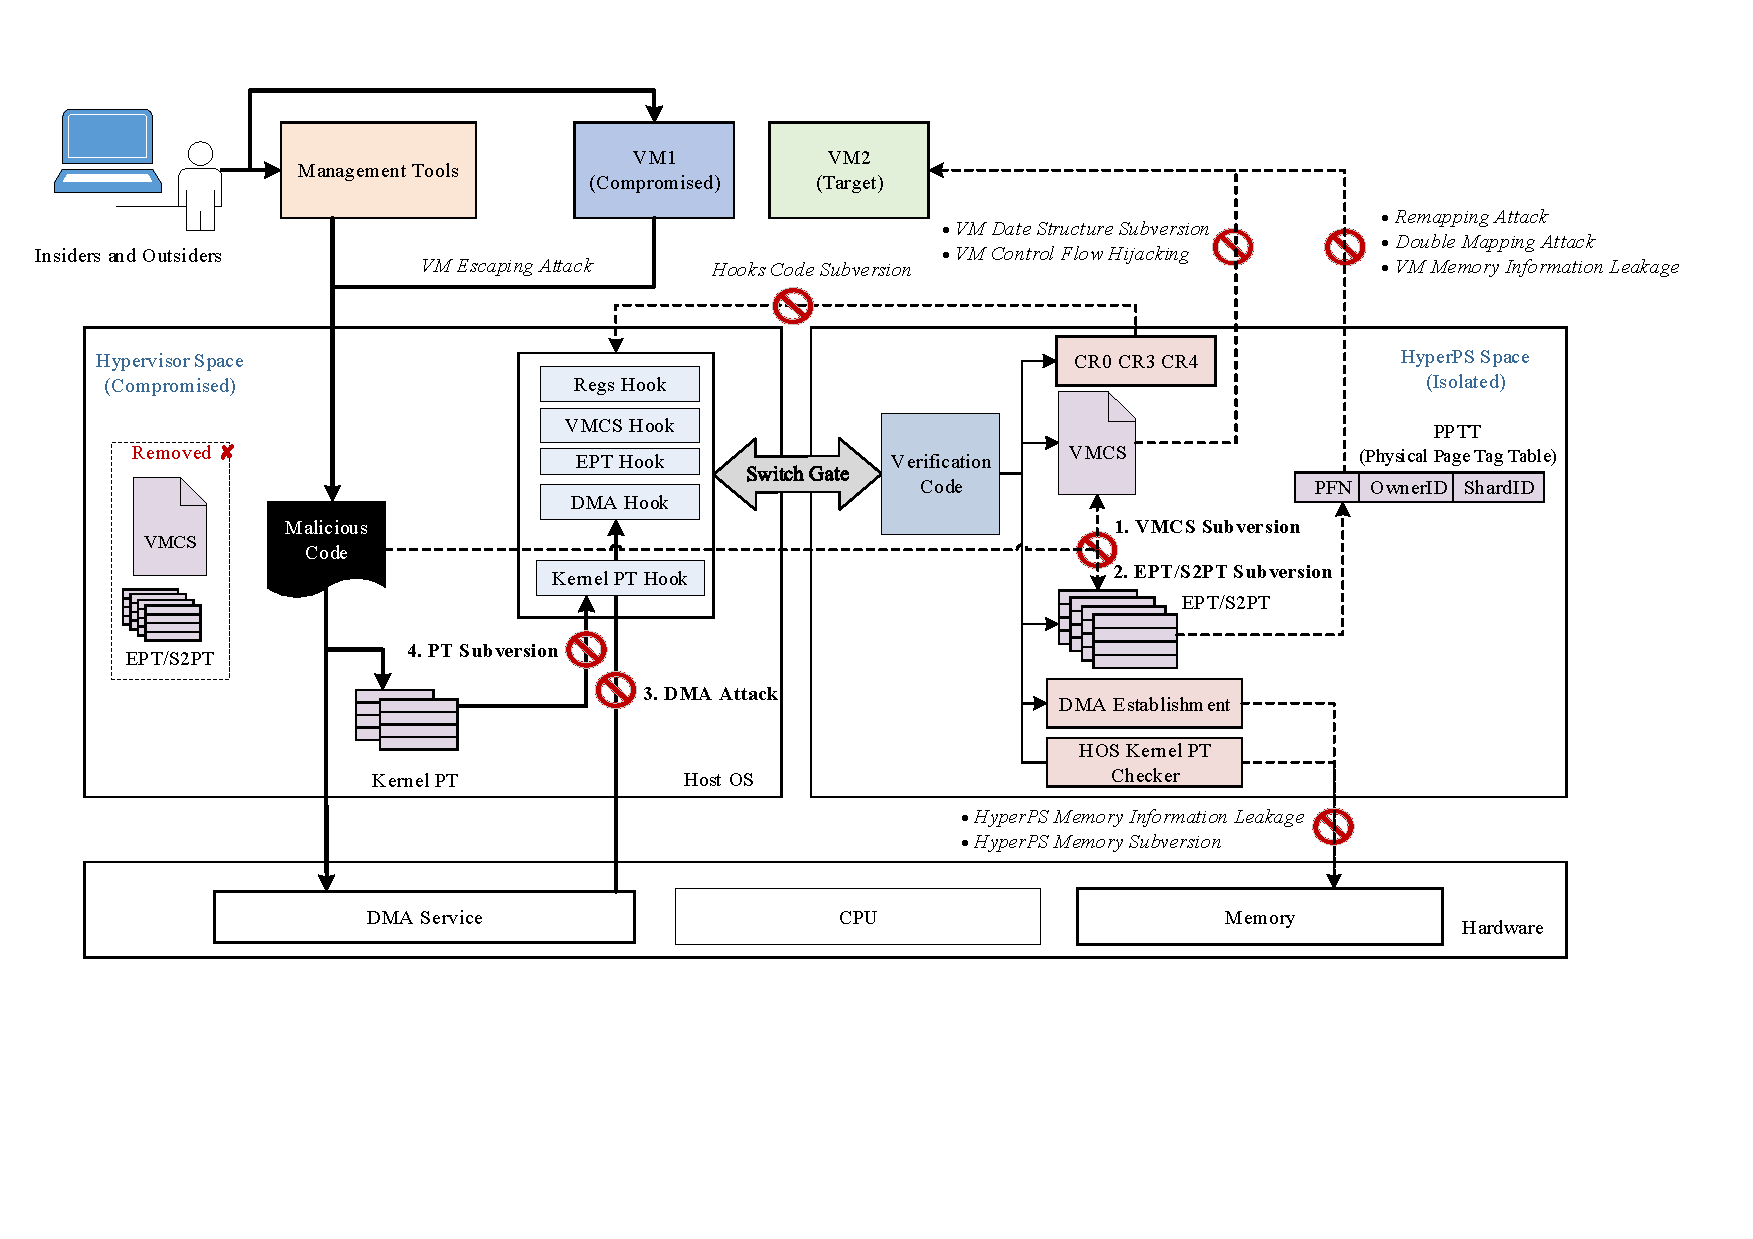
\includegraphics[width=1\textwidth]{IMG/panorama.pdf}
    \caption{The Panorama View of HyperPS. \\ HyperPS is committed to protect guest virtual machine under the compromised HostOS/Hypervisor. Privileges to manage VMCS and EPT are stripped from the compromised HostOS/Hypervisor into a separated and secure execution environment: HyperPS Space. The HyperPS space shares the same processor privilege as the HostOS. HyperPS does not rely on any special hardware or a higher privilege. Updates to VMCS and EPT are abandoned by the HyperPS, if the operations are not authorized or are adjudged as harmful to virtual machine.}
    \label{pic:panorama}
\end{figure*}

\subsection{Motivation} \label{sub:motivation}
In this section, we discuss the motivations of why we need to protect VMs over an untrusted HostOS/Hypervisor.

\iffalse
#######################
###### 写作分析 ####### 
#######################
我们为什么要提出这个观点?首先明白一点:我们是站在VM角度上来思考问题的吗?假如VM不信任下面的VMM,那么就不应该上云,任何安全都不能保证。那么VM租户的角度是否能要求下面提供一个更加安全的架构,应该,但是不应该是租户要求下面的云服务提供商来采用我们的架构,因为一旦是要上云了,人家提供了什么你就选择什么,不能要求其更改云的架构。所以,站的视角一定不是VM租户的角度。那么角度就应该是下面的VMM。就是云服务提供商。对于VMM,其有什么动力要更改他们现在的架构?而不是现在的架构,毕竟无论如何一个同层隔离也更改了现有的云架构了。所以这里不应该假定存在内部攻击者,内部工作人员本身就知道我们的架构的存在,完全可以卸载了就好了,不需要还进行什么防护。所以,只可能存在一种情况,就是云服务提供商也不能完全保证其hostos的安全,但是其最核心的功能应该是如何保证其云的功能是安全的。所以,采用同层隔离的功能将云的相关功能隔离起来。从而实现云部分的安全。换句话说,就是,即使在HostOS存在脆弱点,其已经被攻击者攻陷的前提下,或者上面的VM通过虚拟机逃逸已经获取了下面的os的部分权限的前提下,如何保证VM的安全,即仍然能提供正常的云服务,保证用户的安全。那么前提就是云服务提供商也不完全信任下面的hostOS内核。
这段内容是否是我们的motivation?是,要详细写出来,但是思路不应该说VM租户内容,而应该从后面的内容出发,这个内容要不要在instruction中写出?要,但是要简洁,这里是详细说明。

基于上面的分析,我们假定的威胁模型应该是攻击者可以利用内核的脆弱性,获取了部分hostOS的权限,这权限是什么?这个要详细说明。
首先是最常见的,任意内存读写权限?或者特定的内存的读写权限?能否嵌入shellcode?这些要详细的分析,但是这个部分的工作放到后面,先将motivation写出来。

因为下面的Linux其实有很多脆弱点的,但是在传统的qemu-kvm的框架中,任何
这里首先要讲出如果HostOS并不安全,
The motivation for this work derives directly from
这部分要写出我们为什么要做这个系统,初衷是什么,要解决什么问题。

这部分要写什么?怎么写?
要按照这个逻辑来写:首先最开始用几句话说明云服务提供商最重要的任务是保证上面组会的安全,这是其需要负责的责任。然后需要论证hostos是不安全的,在这个条件下,其云系统可能被危害,一旦HOSTOS被危害,那么就无法保证上面VM的安全,立脚点一定是站在云服务提供商的角度上。最后自然而然的引出我们的motivation,就是如何在hostos被危害的前提条件下,云服务提供商如何保证虚拟机的安全。
\fi





\subsection{Threat Model} \label{sub:thretmodel}
We assume that the HostOS/Hypervisor has been compromised and controlled by the powerful adversary. The adversary can turn off kernel security mechanisms, such as DEP, SMEP, SMAP, and so on. 

%原威胁模型写的有问题。给出的两个例子后面写危害VMCS和
